\documentclass[12pt, twoside]{article}
\usepackage[letterpaper, margin=1in, headsep=0.5in]{geometry}
\usepackage[english]{babel}
\usepackage[utf8]{inputenc}
\usepackage{amsmath}
\usepackage{amsfonts}
\usepackage{amssymb}
\usepackage{tikz}

\usepackage{pgfplots}
\pgfplotsset{width=9cm,compat=1.9}

\usepackage{venndiagram}

\usepackage{graphicx}
\usepackage{enumitem}
\usepackage{multicol}

\usepackage{fancyhdr}
\pagestyle{fancy}
\fancyhf{}
\renewcommand{\headrulewidth}{0pt} % disable the underline of the header

\fancyhead[LE]{\thepage}
\fancyhead[RO]{\thepage \\ Name: \hspace{4cm} \,\\}
\fancyhead[LO]{BECA / Dr. Huson / IB Mathematics\\* Unit 4: Linear functions and regression\\* 6 January 2020}

\begin{document}
\begin{enumerate}
    \subsubsection*{4.3 Do Now Quiz: Graphing linear equations}
    
    \item \begin{enumerate}
        \item Graph and label the two equations. Mark their intersection as an ordered pair.
          \begin{multicols}{2}
            $y =-\frac{3}{4}x-1$ \\
            $x-y=-6$ \hfill (4 pts)
          \end{multicols}     \vspace{1cm}
        \item Find the slopes of the two lines. \hfill (2 points)
          \begin{multicols}{2}
            $m_1=$ \\
            $m_2=$
          \end{multicols}
        \item Why is it incorrect to write $m_1=-\frac{3}{4}x$? \hfill (1 point) \vspace{2cm}
        \item Are the lines parallel, perpendicular, or neither? Justify your answer with an equation or inequality using the slopes. \hfill (2 points)
        \vspace{2cm}
      \end{enumerate}
        \begin{center}
          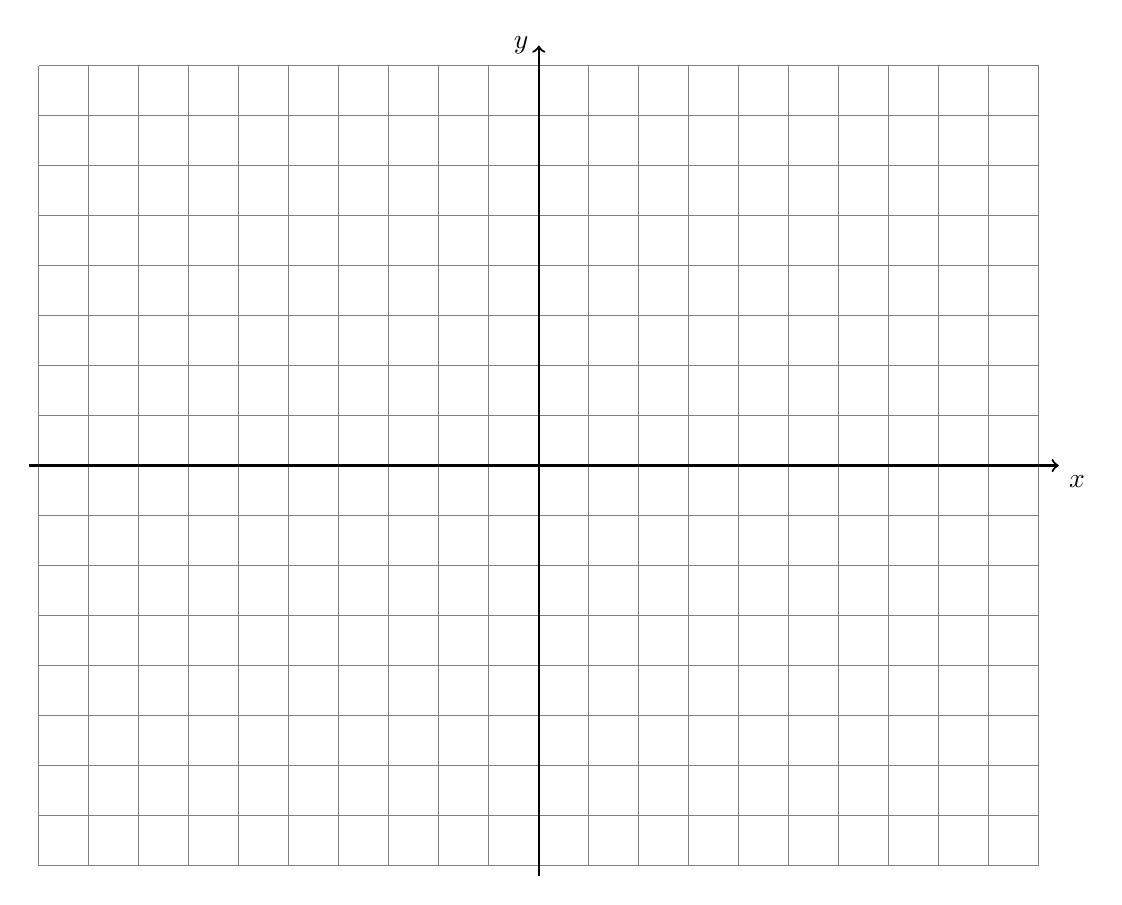
\begin{tikzpicture}[scale=.635]
            \draw [help lines] (-10,-8) grid (10,8);
            \draw [thick, ->] (-10.2,0) -- (10.4,0) node [below right] {$x$};
            \draw [thick, ->] (0,-8.2)--(0,8.4) node [left] {$y$};
          \end{tikzpicture}
        \end{center}
    
\newpage
\subsubsection*{Early finishers: Linear equations, regression}

    \item \begin{enumerate}[itemsep=0.75cm]
    \item A set of six bivariate data are plotted and a linear regression is performed, as shown below. The correlation coefficient, $r$, has the value 0.853.
    \begin{center}
        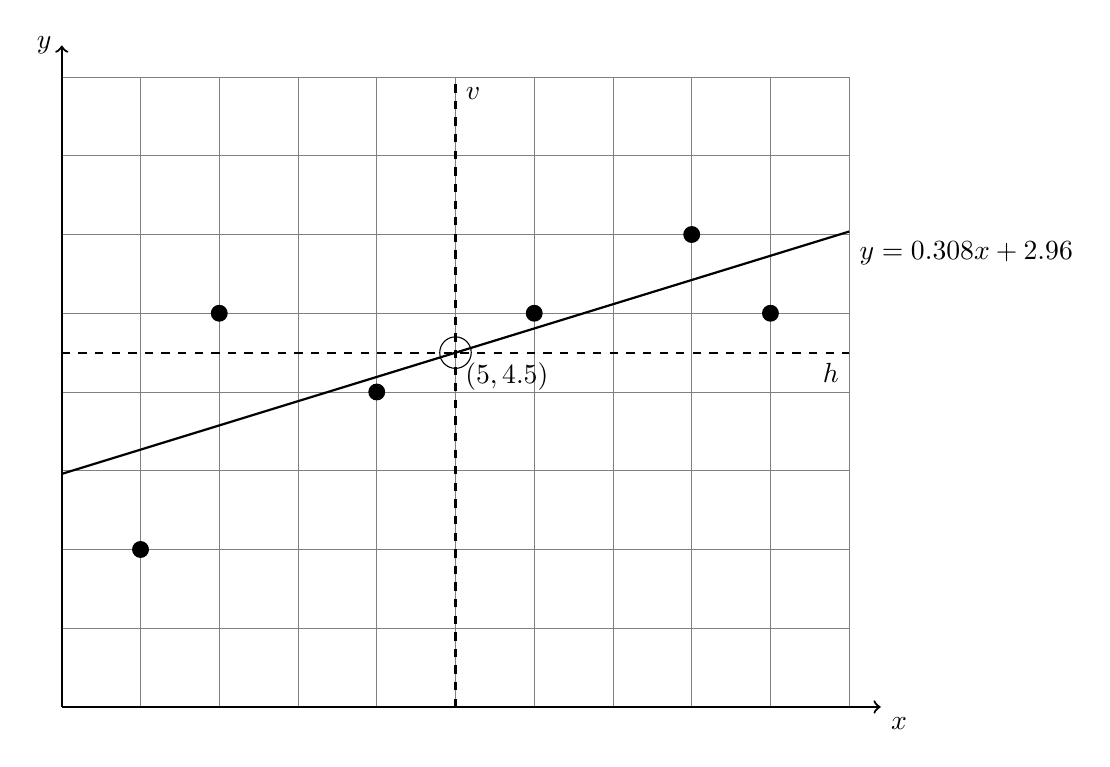
\begin{tikzpicture}%[scale=.635]
        \draw [help lines] (0,0) grid (10,8);
        \draw [thick, ->] (0,0) -- (10.4,0) node [below right] {$x$};
        \draw [thick, ->] (0,0)--(0,8.4) node [left] {$y$};
        \draw [fill] (1,2) circle [radius=0.1];
        \draw [fill] (2,5) circle [radius=0.1];
        \draw [fill] (4,4) circle [radius=0.1];
        \draw [fill] (6,5) circle [radius=0.1];
        \draw [fill] (8,6) circle [radius=0.1];
        \draw [fill] (9,5) circle [radius=0.1];
        \draw [] (5,4.5) circle [radius=0.2]node[below right]{$(5,4.5)$};
        \draw [thick, -] (0,2.96)--(10,6.038) node [below right] {$y=0.308x+2.96$};
        \draw [thick, dashed] (0,4.5)--(10,4.5) node [below left] {$h$};
        \draw [thick, dashed] (5,0)--(5,8) node [below right] {$v$};
        \end{tikzpicture}
    \end{center}
    \item The line of best fit has the equation $y=ax+b$. Write down the value of 
      \begin{enumerate}[itemsep=0.75cm]
      \item $a$: 
      \item $b$:
      \end{enumerate}
    \item Characterize the correlation coefficient, $r$.
    \item A horizontal line, $h$, and vertical line, $v$, intersect at the point $(5,4.5)$. Write down the equation of each line.
    \begin{enumerate}[itemsep=0.75cm]
      \item $h$: 
      \item $v$:
      \end{enumerate}
    \item Circle the representation corresponding to the point $(5,4.5)$.\\[0.5cm]
    $(\sigma, v)$ \hfill $(\overline{x},\overline{y})$ \hfill $(r, r^2)$ \hfill $(a, b)$ \hspace{1cm}
    \end{enumerate}
    
\end{enumerate}
\end{document}